\setcounter{ExampleCounter}{1}

%%% Disjoint %%%
In this section, we will focus on computing probabilities of events involving ``or'' as well as learning the concept of mutually exclusive events. We will also discuss complementary events and their probabilities. 

To start, recall the experiment of drawing one card from a standard deck of cards. Let $J$ denote drawing a Jack, and $Q$ denote drawing a Queen. What is the probability of drawing a Jack? It is, of course, 4/52, and the same goes for the probability of drawing a Queen. Now, what is the probability of drawing a Jack \emph{OR} Queen?  By looking back at the deck of cards, we can see that there are 8 cards that are either Jacks or Queens, so 
\[P(J \ OR \ Q)=\dfrac{8}{52},\]
which happens to be the sum of their individual probabilities.

What about, though, if we wanted to find the probability of drawing a Jack or a diamond?  Could we just add their individual probabilities (4/52 and 13/52, respectively)?  Let's check by looking back at the cards and see which correspond to Jacks or diamonds.
\begin{center}
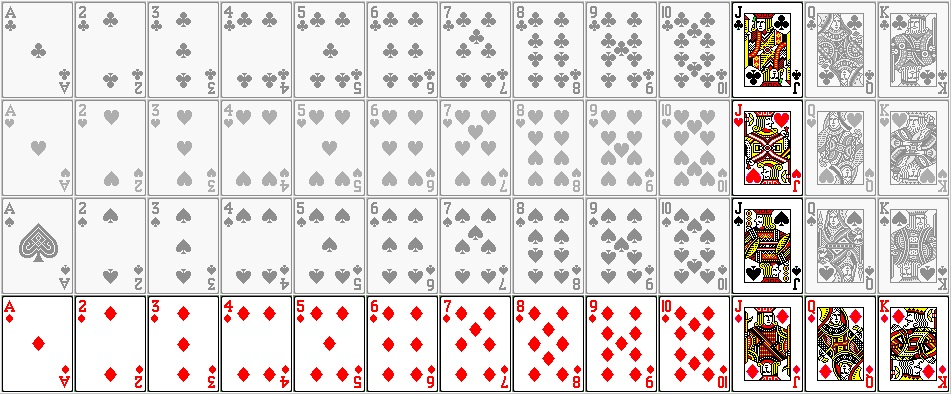
\includegraphics[width=0.8\textwidth]{playingcardsJD}
\end{center}
Notice that there are 16 cards that match that description, so the probability is 16/32, which ISN'T the sum of the individual probabilities.  What went wrong?\\

The answer can be found by looking at the diagram above.  Notice that if we add up the number of Jacks and the number of diamonds (for a total of 17), we \textit{double count} the Jack of diamonds.  This brings us to an important definition that determines how we find the probability of one event OR another occurring: we need to find whether the events are \textbf{mutually exclusive} or \textbf{disjoint}.  That is, can these two events happen at the same time?
\begin{proc}{Disjoint (mutually exclusive) outcomes}
Two outcomes are called \textbf{disjoint} or \textbf{mutually exclusive} if they cannot both happen at the same time.
\end{proc}
Can we draw a card that is both Jack and Queen? Clearly, there is no such card, therefore these events are disjoint. Another familiar example of disjoint events would be getting an even number and getting an odd number when rolling a die. Each number is either even or odd, so these two events are also mutually exclusive.  Above, though, we showed that drawing a Jack and drawing a diamond are NOT mutually exclusive, since you can draw the Jack of diamonds.

Notice that the terms \textbf{disjoint} and \textbf{mutually exclusive}
are equivalent and interchangeable. The Venn diagram below illustrates the concept of mutually exclusive events: two events $A$ and $B$ do not overlap; they are disjoint. 

\begin{center}
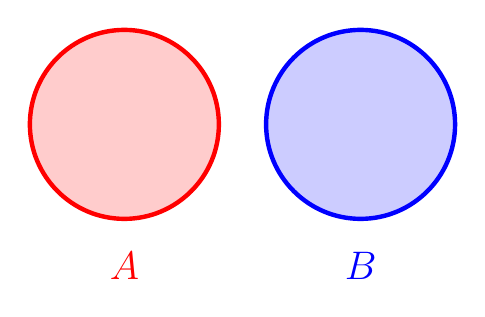
\begin{tikzpicture}
  \draw [ultra thick,color=red, fill=red!20] (-1.5,0) circle (1.2cm);
  \draw [yshift=-1.8cm,xshift=-1.5cm] node {\color{red}\Large $A$};
  
  \draw [ultra thick,color=blue, fill=blue!20] (1.5,0) circle (1.2cm);
  \draw [yshift=-1.8cm,xshift=1.5cm] node {\color{blue}\Large $B$};
\end{tikzpicture}
\end{center}

 Before we formally define a formula for computing probabilities of disjoint events, let us solve some problems by using the rules we already know.


\begin{example}[https://www.youtube.com/watch?v=473To7lQQyI]{Rolling a die}
Suppose you roll a fair six-sided die once. What is the probability of rolling a 6 or an odd number? \\

\marginnote{\bfseries Solution} Since 6 is even, these two events are disjoint, your intuition might tell you to find the probability as follows:
\[ P( O \mbox{ or } 6 ) = P(O) + P(6) = \frac{3}{6} + \frac{1}{6} = \frac{4}{6} = \frac{2}{3} \approx 0.667\]
\end{example}

\begin{try}
If you roll a fair six-sided die once, what is the probability of getting a 5 or a number less than 2? 
\end{try}
\vspace{0.5in}

So, if the events are disjoint, or mutually exclusive, we will be using the formula below: 
\begin{formula}{Addition rule for mutually exclusive events}
If $A_1$ and $A_2$ are mutually exclusive events, then 
 \[  P(A_1 \mbox{ or } A_2) =  P(A_1) +  P(A_2) \]
Furthermore, we can generalize this rule for finitely many disjoint events (where $n$ is the number of events):
\[  P(A_1 \mbox{ or } A_2  \dots \mbox{ or } A_n) =  P(A_1) +  P(A_2) + \dots + P(A_n) \]
\end{formula} 
\vspace{0.5in}

\begin{example}[https://www.youtube.com/watch?v=uD6AB7t_Das]{Drawing a card}
Suppose you draw one card from a standard 52-card deck. What is the probability that you get an Ace or a face card? \\

\marginnote{\bfseries Solution} There are 4 Aces and 12 face cards in a standard deck of cards. These outcomes are disjoint, since only one card is drawn, so we find the probability as follows:
\[ P( A \mbox{ or } F ) = P(A) + P(F) = \frac{4}{52} + \frac{12}{52} = \frac{16}{52} = \frac{4}{13} \approx 0.308\]
\end{example}

\begin{try}
If one card is randomly selected from a deck, what is the probability of getting a number or a red Jack? If one card is randomly selected from a deck, what is the probability of selecting a red suit or a black suit?
\end{try}
\vfill
\pagebreak

\begin{example}[https://www.youtube.com/watch?v=eS3h94W2Lnk]{Marbles}
A large bag contains 28 marbles: 7 are blue, 8 are yellow, 3 are white, and 10 are  red. 
\begin{enumerate}[(a)]
\item If one marble is randomly selected, what is the probability that it is either red or yellow?
\item If one marble is randomly selected, what is the probability that it is neither white nor red?
\end{enumerate}

\begin{center}
\line(1,0){150}
\end{center}

\begin{enumerate}[(a)]
\item Clearly,\marginnote{\bfseries Solution} selecting a red or yellow marble are disjoint events, so we find the probability as follows:
\[ P( R \mbox{ or } Y ) = P(R) + P(Y) = \frac{10}{28} + \frac{8}{28} = \frac{18}{28} = \frac{9}{14} \approx 0.643\]
\item A\sol\ question involving ``neither/nor'' is different from a question involving ``either/or'', because NOT white and NOT red are not mutually exclusive events.  Thus, to answer this question, we will simply count how many marbles are not white and also not red.  This includes the blue and yellow marbles, for a total of $7 + 8 = 15$:
\[P(\textrm{not } W \textrm{ and not } R) = \dfrac{15}{28} \approx 0.54\]
\end{enumerate}
\end{example}

\begin{try}
A bag of M\&M's contains the following candies:  12 are brown, 20 are yellow, 14 are red, 8 are green, and 16 are orange. If one candy is randomly selected, what is the probability that it's either brown or green? 
\end{try}

%%% Not disjoint %%%
What if the events of interest are not mutually exclusive? How do we compute probabilities of events that are not disjoint? Pictorially, we can visualize this situation with the following diagram, where the red intersection of two circles represents all outcomes when two events both happen. For example, if we consider FCC students, selecting a female and selecting a full-time students would not be mutually exclusive events, since there are certainly female students who go to school full time.
\begin{center}
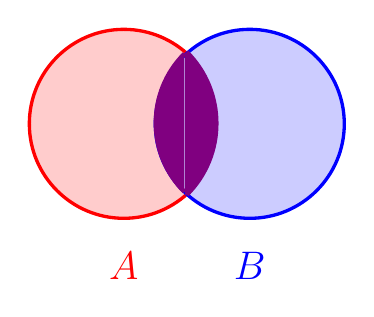
\begin{tikzpicture}
  \draw [very thick,color=red, fill=red!20] (-0.8,0) circle (1.2cm);
  \draw [yshift=-1.8cm,xshift=-0.8cm] node {\color{red}\Large $A$};
  
  \draw [very thick,color=blue, fill=blue!20] (0.8,0) circle (1.2cm);
  \draw [yshift=-1.8cm,xshift=0.8cm] node {\color{blue}\Large $B$};
  
  \draw [ultra thick,color=blue!50!red, fill=blue!50!red] (0,-0.9) arc (-45:45:1.28cm);
  \draw [ultra thick,color=blue!50!red, fill=blue!50!red] (-0.03,0.89) arc (135:225:1.24cm);
  \draw [ultra thick,color=blue!50!red] (0,-0.9) -- (0,0.9);
\end{tikzpicture}
\end{center}

Let's go back to the deck of cards to see how to calculate probabilities in situations like this.  We'll again use the example of drawing a Jack or a diamond.
\vspace{0.1in}

\begin{center}
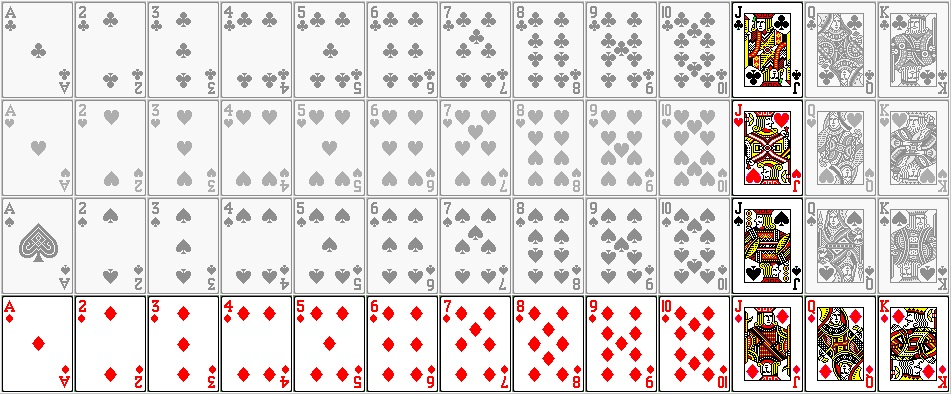
\includegraphics[width=0.8\textwidth]{playingcardsJD}
\end{center}
\vspace{0.1in}

As we noted already, these are not mutually exclusive events.  Because of that, adding the probability of drawing a Jack (4/52) and the probability of drawing a diamond (13/52) gave an incorrect answer of 17/52, where the correct probability--as we noted earlier--is 16/52.  Again, this is because we \textit{double counted} the Jack of diamonds, once when we calculated the probability of drawing a Jack and once when we calculated the probability of a diamond.

The way to correct for this double counting is to subtract off the overlap; thus, we'll add up the probability of drawing a Jack and the probability of drawing a diamond, and then subtract the probability of drawing both together (i.e. of drawing the Jack of diamonds):
\[P(J \ OR \ D) = P(J)+P(D)-P(JD) = \dfrac{4}{52}+\dfrac{13}{52}-\dfrac{1}{52} = \dfrac{16}{52}\]
\vfill

In general, to calculate probabilities of compound events that are not mutually exclusive, we will use the General Addition rule:
\vfill

\begin{formula}{General Addition rule}
If $A_1$ and $A_2$ are any events, then 
 \[  P(A_1 \mbox{ or } A_2) =  P(A_1) +  P(A_2) - P( A_1 \mbox{ and } A_2 ) \]
\end{formula}
\vfill

Notice that this is a more general form of the addition rule we stated earlier, with mutually exclusive events.  If two events are mutually exclusive, the probability of them occurring together is 0, so the general addition rule simplifies down in that case to the simpler addition rule.
\vfill
 
\begin{example}[https://www.youtube.com/watch?v=lx7DRG6N1r8]{Drawing a card}
Suppose you draw one card from a standard 52-card deck. What is the probability that you get a King or a spade? \\

\marginnote{\bfseries Solution} There are 4 Kings and 13 spades, where one of these cards is a King of spades. Drawing the King of spades means both events happen at the same time, so these events are not mutually exclusive. To compute the probability correctly, we need to make sure we don't ``double count'' any of the outcomes, and in this case it is drawing the King of spades. Applying the general addition rule, we get
\[ P( K \mbox{ or } S ) = P(K) + P(S) - P(K \mbox{ and } S)  = \frac{4}{52} + \frac{13}{52} - \frac{1}{52}  = \frac{16}{52} = \frac{4}{13} \approx 0.308\]
By subtracting $P(K \mbox{ and } S)$, we guarantee that we count the King of Spades only once.
\end{example}

\begin{try}
Suppose you draw one card from a standard 52-card deck. What is the probability that you get a Queen or a face card? 
\end{try}
\vfill
\pagebreak

Let's take a look at a slightly different example of events that are not disjoint.

\begin{example}[https://www.youtube.com/watch?v=Z3FKbz7RnSs]{FCC students}
Consider the following information about a group of 130 FCC students:

\begin{center}
\begin{tabular}{|c|c|c|c|}
\hline
Gender & Right-handed & Left-handed & \textbf{Total} \\ \hline 
Female & 58 & 13 & 71\\ \hline
Male & 47 & 12 & 59  \\ \hline
\textbf{Total} & 105 & 25 & 130 \\ \hline 
\end{tabular}
\end{center}

If one person is randomly selected from the group, what is the probability this student is female or left-handed? \\

\marginnote{\bfseries Solution} These events are not disjoint, since there are 13 females who are left-handed. Thus, we apply the general addition formula:
\[  P(F \mbox{ or } L) = \frac{71}{130} + \frac{25}{130} - \frac{13}{130} = \frac{83}{130} \approx 0.638 \]
Notice that the only students not ``qualifying'' for the event of interest are right-handed males. There are 47 of them, and 130 - 47 = 83. 
\end{example}

\begin{try}
Using the example above, compute the probability of selecting a male or a right-handed student. 
\end{try}

\begin{example}[https://www.youtube.com/watch?v=QE9xCoQBclw]{Speeding tickets and car color} 
The table below shows the number of survey subjects who have received a speeding ticket in the last year and those who have not received a speeding ticket, as well as the color of their car. Find the probability that a randomly chosen person has a red car \emph{or} got a speeding ticket
\begin{center}
\begin{tabular}{|c|c|c|c|}
\hline
 & Speeding ticket & No speeding ticket& \textbf{Total} \\ \hline 
Red car & 15 & 135 & 150\\ \hline
Not red car & 45 & 470 & 515  \\ \hline
\textbf{Total} & 60 & 605 & 665 \\ \hline 
\end{tabular}
\end{center}	

\marginnote{\bfseries Solution} Notice that having a red car and getting a speeding ticket are not mutually exclusive events, since 15 people had both. Thus, we perform the following computations: \\

\emph{P(red car) + P(got a speeding ticket) $-$ P(red car and got a speeding ticket)} 

\[  \frac{150}{665} + \frac{60}{665} - \frac{15}{665}  = \frac{195}{665}  \approx 0.293\]
\end{example}

\begin{try}
A local fitness club conducted a survey about the type of workouts their members prefer, and the results are recorded in the table below.
\begin{center}
\begin{tabular}{|c|c|c|c|}
\hline
 & Cardio exercises & Strength training& \textbf{Total} \\ \hline 
Female & 45 & 16 & 61 \\ \hline
Male & 27 & 82 & 109  \\ \hline
\textbf{Total} & 72 & 98 & 170 \\ \hline 
\end{tabular}
\end{center}
If one person is randomly selected from this group, what is the probability of selecting a male or a member who prefers cardio exercise?
\end{try}
\pagebreak

\subsection{Complements}
The probability of an event not occurring can be just as useful as computing the probability of that event happening. The best way to introduce this concept is to consider an example. Let's revisit the standard 52-card deck, where we randomly select one card:

\begin{center}
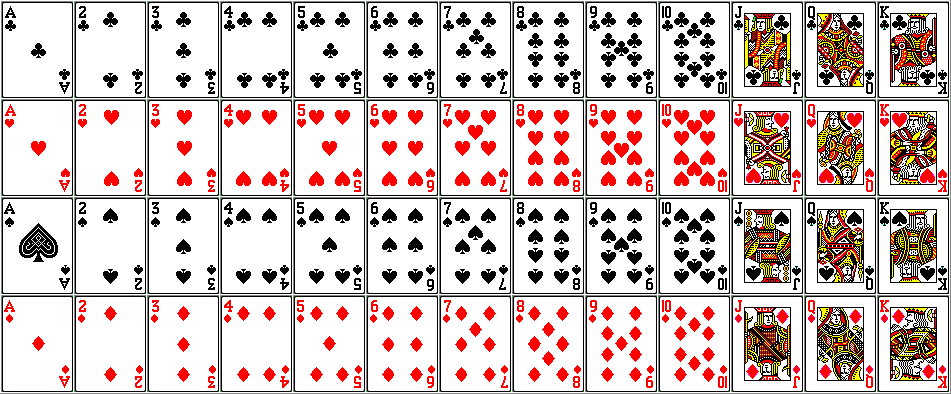
\includegraphics[width=0.8\textwidth]{playingcards}
\end{center}

What is the probability of not drawing an Ace? Well, you know that there are 4 Aces in the deck, so $52 - 4 = 48$ cards that are not Aces. We compute:
\[ P(\mbox{ not } \mbox{ Ace }) = \frac{48}{52} \approx 0.923 \]
Now, notice that 
\[  \frac{48}{52} = 1 - \frac{4}{52}, \mbox{ where } P(Ace) = \frac{4}{52}\]
This is not a coincidence. If you recall the basic rules of probability, the sum of the probabilities of all outcomes must be 1. In this case, the card you draw is either Ace or it's not, so it makes sense that the probabilities of these two events add up to 1. 
%%% NOT %%%

\begin{formula}{Complement of an event}
The complement of an event $A$  is denoted by $A^c$ and represents all outcomes not in $A$. 
\begin{enumerate}
	\item $P(A) + P(A^c) = 1 $
	\item $P(A) = 1 - P(A^c) $ 
	\item $P(A^c) = 1 - P(A) $ 
\end{enumerate}
\end{formula}
\vspace{-0.15in}

\begin{example}[https://www.youtube.com/watch?v=YpjdHUsKaow]{Not hearts!}
If you pull a random card, what is the probability it is not a
heart? \\

\marginnote{\bfseries Solution} There are 13 hearts in the deck, so $P(\mbox{hearts}) = \frac{13}{52} = \frac{1}{4}$. The probability of not drawing a heart is the complement:
\[  P(\mbox{not hearts} ) = 1 - P(\mbox{hearts}) = 1 - \frac{1}{4} = \frac{3}{4} \]
\end{example}

\begin{try}
If you pull a random card, what is the probability it is not a
face card?
\end{try} 
\pagebreak

Let's consider an example that might be more relevant to you as a student: 

\begin{example}[https://www.youtube.com/watch?v=munZCN0L2uA]{Multiple choice question}
A multiple choice question has 5 answers, and exactly one of them is correct. If you were to guess, what is the probability of not getting the correct answer? \\

\marginnote{\bfseries Solution} Since only one of the answers is correct, we have $P(\mbox{correct}) = \frac{1}{5}$, so
\[  P(\mbox{not correct}) = 1 - P(\mbox{correct}) = 1 - \frac{1}{5} = \frac{4}{5} = 0.8 \]
\end{example}

\begin{try}
A multiple choice question has 6 answers, and exactly two of them are correct. If you were to guess, what is the probability of not getting the correct answer?  If a test has 4 questions with 6 possible answers, what is the probability of not getting any of the questions correct? (\emph{You are technically not ready to answer this part of the question just yet, but it is a good exercise to think about!})
\end{try}

\begin{example}[https://www.youtube.com/watch?v=ICbVL7wFRYU]{FCC students' demographics}
According to the FCC website, female students made up 57\% of the Fall 2014 student body. If one student is randomly selected, what is the probability the student is not female? \\

\marginnote{\bfseries Solution} The probability of selecting a female student is 0.57, thus using the complement rule, we compute:
\[ P(\mbox{not female}) = 1 - P(\mbox{female}) = 1 - 0.57 = 0.43 \]
\end{example}

\begin{try}
According to the FCC website, full-time students made up 34\% of the fall 2014 student body. If one student is randomly selected, what is the probability the student is not full-time? \\
\end{try}
\vfill
\pagebreak

\begin{exercises}
\ptwo{A jar contains 6 red marbles numbered 1 to 6 and 8 blue marbles numbered 1 to 8. A marble is drawn at random from the jar. Find the probability the marble is red or odd-numbered.}
\ptwo{A jar contains 4 red marbles numbered 1 to 4 and 10 blue marbles numbered 1 to 10. A marble is drawn at random from the jar. Find the probability the marble is blue or even-numbered.}

\ptwo{ You draw one card from a standard 52-card deck. 
\begin{enumerate}
\item What is the probability of selecting a King or a Queen?
\item What is the probability of selecting a face card or a 10?
\item What is the probability of selecting a spade or a heart?
\item What is the probability of selecting a red card or a black card?
\end{enumerate}}
\ptwo{  You are dealt a single card from a standard 52-card deck.
\begin{enumerate}
\item Find the probability that you are not dealt a diamond.
\item Find the probability that you are not dealt a face card.
\item Find the probability that you are not dealt an Ace.
\item Find the probability that you are not dealt a jack or a king.
\end{enumerate}}

\pone{Consider the following information about a group of 130 FCC students:
\begin{center}
\begin{tabular}{|c|c|c|c|}
\hline
Gender & Right-handed & Left-handed & \textbf{Total} \\ \hline 
Female & 58 & 13 & 71\\ \hline
Male & 47 & 12 & 59  \\ \hline
\textbf{Total} & 105 & 25 & 130 \\ \hline 
\end{tabular}
\end{center}
If one person is randomly selected from the group, what is the probability this student is female or left-handed?}

\pone{The table below shows the number of survey subjects who have received and not received a speeding ticket in the last year, and the color of their car. Find the probability that a randomly chosen person has a red car \emph{or} got a speeding ticket. 


\begin{center}
\begin{tabular}{|c|c|c|c|}
\hline
 & Speeding ticket & No speeding ticket& \textbf{Total} \\ \hline 
Red car & 15 & 135 & 150\\ \hline
Not red car & 45 & 470 & 515  \\ \hline
\textbf{Total} & 60 & 605 & 665 \\ \hline 
\end{tabular}
\end{center}
}

\ptwo{\small Suppose you roll a blue six sided die and a red six sided die, and add their totals.
Find the probability of rolling:

\begin{enumerate}
	\item a 7 or 11
  \item an even number or a number less than 6
  \item a prime number or a number greater than 5
\end{enumerate}}
\ptwo{A bag contains 4 white counters, 6 black counters, and 1 green counter. What is the
probability of drawing:
\begin{enumerate}
	\item A white counter or a green counter?
  \item A black counter or a green counter?
  \item Not a green counter?
\end{enumerate}}

\pone{ A poll was taken of 14,056 working adults aged 40-70 to determine their level of
education. The participants were classified by sex and by level of education. The results
were as follows.

\begin{center}
\begin{tabular}{c|cc|c} \hline
Education Level     &  Male &  Female &  Total \\ \hline
High School or Less & 3141  &2434     &  5575  \\ 
Bachelor's Degree   & 3619  &3761     &  7380  \\
Master's Degree     & 534   &472      &  1006  \\
Ph.D.               & 52    &43       &  95    \\ \hline
Total 							& 7346  &6710     & 14,056 \\ 
\end{tabular}
\end{center}
A person is selected at random. Compute the following probabilities:

\begin{enumerate}
	\item probability that the selected person does not have a Ph.D.
	\item probability that the selected person does not have  a Master's degree
	\item probability that the selected person is female or has a  Master's degree
	\item probability that the selected person is male or has a Ph.D 
\end{enumerate}}

\end{exercises}